\documentclass{seuthesis}

\newcommand{\demobox}[2]{\fbox{\rule{0pt}{#2}\rule{#1}{0pt}}}

\addkey{机器学习}{ML}
\addkey{关键词 2}{Keyword2}
\addkey{关键词 3}{Keyword3}
\addkey{关键词 4}{Keyword4}

\seusetup{
  title                          = {二号黑体居中},
  subtitle                       = {（如此行空白，可自行删除）},
  author                         = {},
  student_id                     = {},
  school                         = {},
  major                          = {},
  supervisor                     = {},
  date_range                     = {},
  cover_date                     = {2025 年\hspace{0.95em}月\hspace{0.95em}日},
  originality_date               = {},
  authorization_author_date      = {},
  authorization_supervisor_date  = {},
  ai_subject                     = {},
  ai_used                        = unset,
  ai_student_date                = {},
  ai_teacher_date                = {},
  ai_teacher_comment             = {}
}

\begin{document}

\seumakefrontmatter

\seuprefacematter
\seumakechineseabstract
\seumakeenglishabstract
\seumaketableofcontents

\seumainmatter
\input{content/chapter1.tex}
\chapter{第二章标题}

具体研究内容每一章应另起页书写，层次要清楚，内容要有逻辑性，每一章标题需要按论文实际研究内容进行填写，
不可直接写成第二章 正文。研究内容因学科、选题特点可有差异，但必须言之成理，论据可靠，严格遵循本学科国际通行的学术规范。

中文为小四号宋体，英文及数字为小四号 Times New Roman，首行缩进 2 个字符，行间距为 1.5 倍。

\section{插图格式要求}

插图力求精炼，且每个插图均应有图序和图名。图序与图名位于插图下方，图序一般按章节编排，
如图 1-1（第一章第 1 个图），在插图较少时可以全文连续编序，如图 10。

如一个插图由两个及以上的分图组成，分图用(a)、(b)、(c)等标出，并标出分图名。
简单文字图可用 WORD 直接绘制，复杂的图考虑使用相应的图形绘制软件完成，以提高图形表达质量。

插图居中排列，与上文文本之间空一行。图序图名设置为五号宋体居中，图序与图名之间空一格。

\begin{figure}[htbp]
  \centering
  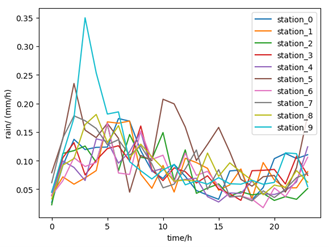
\includegraphics[width=0.70\linewidth]{imgs/demo1.png}
  \caption{每小时降水量 24 小时均值分布图}
\end{figure}

\clearpage

\begin{figure}[htbp]
  \centering
  \begin{subfigure}[b]{0.38\textwidth}
    \centering
    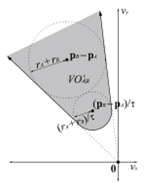
\includegraphics[width=0.88\linewidth]{imgs/demo2(a).png}
    \caption*{(a) 速度障碍集合}
  \end{subfigure}
  \hfill
  \begin{subfigure}[b]{0.38\textwidth}
    \centering
    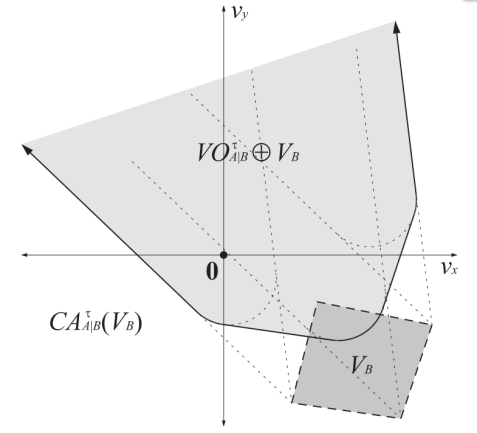
\includegraphics[width=0.88\linewidth]{imgs/demo2(b).png}
    \caption*{(b) 避免碰撞集合}
  \end{subfigure}
  \caption{速度障碍法速度选择}
\end{figure}

\section{表格格式要求}

表格的结构应简洁，一律采用三线表，应有表序和表名，且表序和表名位于表格上方。表格可以逐章单独编序（如：表 2.1），
也可以统一编序（如：表 10），采用哪种方式应和插图及公式的编序方式统一。表序必须连续，不得重复或跳跃。

表格无法在同一页排版时，可以用续表的形式另页书写，续表需在表格右上角表序前加“续”字，如“续表 2.1”，并重复表头。

表格居中，边框为黑色直线 1 磅，中文为五号宋体，英文及数字为五号 Times New Roman 字体，表序与表名之间空一格，
表格与下文之间空一行。

\begin{table}[htbp]
  \centering
  \caption{降水率分级统计}
  \begin{tabular}{cccc}
    \toprule
    降水率(mm/h)分级 & 该等级所占比例(\%) & \multicolumn{2}{c}{降水等级描述} \\
    \midrule
    $0 \le x < 0.5$     & 90.36 & \multicolumn{2}{c}{没有雨或雨很小} \\
    $0.5 \le x < 2.0$   & 6.41  & \multicolumn{2}{c}{小雨} \\
    $2.0 \le x < 5.0$   & 2.04  & \multicolumn{2}{c}{中雨} \\
    $5.0 \le x < 10.0$  & 0.10  & \multicolumn{2}{c}{大雨} \\
    $10.0 \le x < 30.0$ & 0.73  & \multicolumn{2}{c}{大雨到暴雨} \\
    $30.0 \le x < 100.0$ & 0.16 & \multicolumn{2}{c}{暴雨} \\
    \bottomrule
  \end{tabular}
\end{table}

\begin{table}[htbp]
  \centering
  \caption{室外细菌气溶胶香农-维纳指数（H）和均匀性指数（E）}
  \begin{tabular}{lcccccccccccc}
    \toprule
    & \multicolumn{4}{c}{Stage 1 (>7.1 $\mu$m)} & \multicolumn{4}{c}{Stage 2 (4.8-7.1 $\mu$m)} & \multicolumn{4}{c}{Stage 3 (3.2-4.7 $\mu$m)} \\
    \cmidrule(lr){2-5}\cmidrule(lr){6-9}\cmidrule(lr){10-13}
    & Con & Low & Medium & High & Con & Low & Medium & High & Con & Low & Medium & High \\
    \midrule
    H & 2.52 & 2.58 & 2.57 & 2.24 & 2.48 & 2.21 & 2.21 & 2.36 & 2.66 & 2.65 & 2.64 & 2.53 \\
    E & 0.87 & 0.88 & 0.93 & 0.85 & 0.90 & 0.86 & 0.86 & 0.85 & 0.90 & 0.90 & 0.85 & 0.88 \\
    \bottomrule
  \end{tabular}
\end{table}

\begin{table}[htbp]
  \centering
  \caption{统计表}
  \begin{tabular}{ccccc}
    \toprule
    产品 & 产量 & 销量 & 产值 & 比重 \\
    \midrule
    手机 & 11000 & 10000 & 500 & 50\% \\
    电视机 & 5500 & 5000 & 220 & 22\% \\
    计算机 & 1100 & 1000 & 280 & 28\% \\
    合计 & 17600 & 16000 & 1000 & 100\% \\
    \bottomrule
  \end{tabular}
\end{table}

\begin{table}[htbp]
  \centering
  \caption{分栏表}
  \begin{tabular}{ccccc}
    \toprule
    年度 & 产品 & 产量 & 销量 & 产值 \\
    \midrule
    \multirow{2}{*}{2004} & 手机 & 11000 & 10000 & 500 \\
      & 计算机 & 1100 & 1000 & 280 \\
    \multirow{2}{*}{2005} & 手机 & 16000 & 13000 & 550 \\
      & 计算机 & 2100 & 1500 & 320 \\
    \bottomrule
  \end{tabular}
\end{table}

\section{表达式}

论文中的公式应注序号并加圆括号，序号一律用阿拉伯数字连续编序（如（28））或逐章编序（如（3.6）），
编号方式应与插图、表格方式一致。序号排在版面右侧，且距右边距离相等。公式与序号之间不加虚线。

长公式在一行无法写完的情况下，原则上应在等号（或数学符号，如“+”、“-”号）处换行，数学符号在换行的行首。
公式及文字中的一般变量（或一般函数）（如坐标 $X$、$Y$，电压 $V$，频率 $f$）宜用斜体，
矢量用粗斜体如 $\bm{S}$ 或白斜体上加单箭头，常用函数（如三角函数 $\cos$、对数函数 $\ln$ 等）、
数字运算符、化学元素符号及分子式、单位符号、产品代号、人名地名的外文字母等用正体。

公式排版时可选中模板中的“公式式样”，先将光标移至公式前，按“Tab”键，公式居中；
再将光标移至编号前，按“Tab”键移动一个制表符位置，使公式编号右对齐。

\clearpage

\begin{equation}
  V_{\text{cell}} = E_{\text{OCV}} - V_{\text{act}} - V_{\text{ohm}} - V_{\text{conc}}
\end{equation}

\begin{equation}
  \begin{aligned}
    E_{\text{OCV}} ={}& 1.229 - 0.85 \times 10^{-3}(T_{\text{st}} - T_0) \\
    & + 4.3085 \times 10^{-5} T_{\text{st}}
    \left[
      \ln \left( \frac{P_{H_2}}{1.01325} \right)
      + \frac{1}{2}\ln \left( \frac{P_{O_2}}{1.01325} \right)
    \right]
  \end{aligned}
\end{equation}

\section{注释}

正文中有个别名词或情况需要解释时，可加注说明，注释采用页末注（将注文放在加注页的下端）。
在引文的右上角标注序号 \ding{172}、\ding{173}、……，如“马尔可夫链\footnote{马尔可夫链表示……}”。
若在同一页中有两个以上的注时，按各注出现的先后，顺序编号。引文序号，以页为单位，
且注释只限于写在注释符号出现的同页，不得隔页。

注释采用小五号宋体，英文及数字为小五号 Times New Roman 字体，利用“引用”插入脚注功能插入。

\input{content/chapter3.tex}

\seuprintbibliography

\appendix
\input{content/appendix-a.tex}
\input{content/acknowledgements.tex}

\seumottopage

\end{document}
